%\documentclass[prd,twocolumn,aps,psfig,showpacs,nofootinbib,nobibnotes,superscriptaddress,preprintnumbers,times]{revtex4}
\documentclass[prd,twocolumn,aps,psfig,nofootinbib,nobibnotes,superscriptaddress,preprintnumbers,times]{revtex4-2}
%\documentclass[prd,aps,psfig,nofootinbib,nobibnotes,superscriptaddress,preprintnumbers,times]{revtex4-2}\setlength{\topmargin}{-14mm}
\usepackage{graphicx,bm,color,amsmath,amssymb, mathtools,subcaption}
\graphicspath{{./fig/}}
\captionsetup{justification   = RaggedRight,
              singlelinecheck = false}

\usepackage[hidelinks]{hyperref}
%\hypersetup{
%  colorlinks   = true, %Colours links instead of ugly boxes
%  urlcolor     = blue, %Colour for external hyperlinks
%  linkcolor    = red, %Colour of internal links
%  citecolor    = blue %Colour of citations
%}
\hypersetup{
  colorlinks   = true, %Colours links instead of ugly boxes
  urlcolor     = [RGB]{46,48,146}, %Colour for external hyperlinks
  linkcolor    = [RGB]{46,48,146}, %Colour of internal links
  citecolor    = [RGB]{46,48,146} %Colour of citations
}

\def\red{\textcolor{red}}
\def\blue{\textcolor{blue}}

\usepackage{braket,orcidlink}

\usepackage{relsize}

%|||||||||||||||||||||||||||||||||||||||||||||||||||||||||||||||||||
%             Customized Commands
%|||||||||||||||||||||||||||||||||||||||||||||||||||||||||||||||||||
%  mathematical abbreviations
%
%
%
\newcommand{\BoldVec}[1]{\mathchoice%
  {\mbox{\boldmath $\displaystyle     #1$}}%
  {\mbox{\boldmath $\textstyle        #1$}}%
  {\mbox{\boldmath $\scriptstyle      #1$}}%
  {\mbox{\boldmath $\scriptscriptstyle#1$}}%
}
%\newcommand{\BoldVec}[1]{\bm{#1}}}
%
% math debs
\newcommand{\EQ}{\begin{equation}}
\newcommand{\EN}{\end{equation}}
\newcommand{\EQA}{\begin{eqnarray}}
\newcommand{\ENA}{\end{eqnarray}}
\newcommand{\eq}[1]{(\ref{#1})}
\newcommand{\EEq}[1]{Equation~(\ref{#1})}
\newcommand{\Eq}[1]{Eq.~(\ref{#1})}
\newcommand{\Eqs}[2]{Eqs~(\ref{#1}) and~(\ref{#2})}
\newcommand{\EEqs}[2]{Equations~(\ref{#1}) and~(\ref{#2})}
\newcommand{\eqs}[2]{(\ref{#1}) and~(\ref{#2})}
\newcommand{\Eqss}[2]{Eqs~(\ref{#1})--(\ref{#2})}
%\newcommand{\Sec}[1]{\S\,\ref{#1}}
%\newcommand{\Secs}[2]{\S\S\,\ref{#1} and~\ref{#2}}
\newcommand{\Sec}[1]{Sec.~\ref{#1}}
\newcommand{\Secs}[2]{Secs.~\ref{#1} and~\ref{#2}}
\newcommand{\App}[1]{Appendix~\ref{#1}}
\newcommand{\Fig}[1]{Fig.~\ref{#1}}
\newcommand{\FFig}[1]{Figure~\ref{#1}}
\newcommand{\Tab}[1]{Table~\ref{#1}}
\newcommand{\Figs}[2]{Figs.~\ref{#1} and \ref{#2}}
\newcommand{\Tabs}[2]{Tables~\ref{#1} and \ref{#2}}
%\newcommand{\bra}[1]{\langle #1\rangle}
\newcommand{\bbra}[1]{\left\langle #1\right\rangle}
\newcommand{\mean}[1]{\overline #1}
\newcommand{\meanB}{\overline{B}}
\newcommand{\meanC}{\overline{C}}
\newcommand{\meanU}{\overline{U}}
\newcommand{\meanW}{\overline{W}}
\newcommand{\meanPhi}{\overline{\Phi}}
\newcommand{\meanF}{\overline{\cal F}}
\newcommand{\meanR}{\overline{\cal R}}
\newcommand{\meanAA}{\overline{\bm{A}}}
\newcommand{\meanBB}{\overline{\bm{B}}}
\newcommand{\meanEE}{\overline{\bm{E}}}
\newcommand{\meanUU}{\overline{\bm{U}}}
\newcommand{\meanWW}{\overline{\bm{W}}}
\newcommand{\meanJJ}{\overline{\mbox{\boldmath $J$}}}
\newcommand{\meanuu}{\overline{\mbox{\boldmath $u$}}}
\newcommand{\meanGG}{\overline{\mbox{\boldmath $G$}}}
\newcommand{\meanAB}{\overline{\mbox{\boldmath $A\cdot B$}}}
\newcommand{\meanAoBo}{\overline{\mbox{\boldmath $A_0\cdot B_0$}}}
\newcommand{\meanApoBpo}{\overline{\mbox{\boldmath $A'_0\cdot B'_0$}}}
\newcommand{\meanApBp}{\overline{\mbox{\boldmath $A'\cdot B'$}}}
\newcommand{\meanuxB}{\overline{\mbox{\boldmath $\delta u\times \delta B$}}}
\newcommand{\meanemfs}{\overline{\cal E} {}}
\newcommand{\meanemf}{\overline{\mbox{\boldmath ${\cal E}$}} {}} %redundant
\newcommand{\meanAAAA}{\overline{\mbox{\boldmath ${\mathsf A}$}} {}}
\newcommand{\meanSSSS}{\overline{\mbox{\boldmath ${\mathsf S}$}} {}}
\newcommand{\meanAAA}{\overline{\mathsf{A}}}
\newcommand{\meanSSS}{\overline{\mathsf{S}}}
\newcommand{\meanCC}{\overline{\mbox{\boldmath ${\cal C}$}} {}}
\newcommand{\meanFF}{\overline{\mbox{\boldmath ${\cal F}$}} {}}
\newcommand{\meanRR}{\overline{\mbox{\boldmath ${\cal R}$}} {}}
\newcommand{\calFF}{\overline{\mbox{\boldmath ${\cal F}$}} {}}
\newcommand{\meanEMF}{\overline{\mbox{\boldmath ${\cal E}$}} {}}
\newcommand{\tildeFFFF}{\tilde{\mbox{\boldmath ${\cal F}$}}{}}{}
\newcommand{\hatFFFF}{\hat{\mbox{\boldmath ${\cal F}$}}{}}{}
\newcommand{\meanFFFF}{\overline{\mbox{\boldmath ${\cal F}$}}{}}{}
\newcommand{\meanFFF}{\overline{\cal F}}
\newcommand{\hatOO}{\hat{\bm{\Omega}}}
\newcommand{\hatAA}{\hat{\bm{A}}}
\newcommand{\hatBB}{\hat{\bm{B}}}
\newcommand{\tildeh}{\tilde{h}}
\newcommand{\tildeT}{\tilde{T}}
\newcommand{\tildehhh}{\tilde{\sf h}}
\newcommand{\tildeTTT}{\tilde{\sf T}}
%
% tilde
%
\newcommand{\eee}{{\sf e}}
\newcommand{\hhh}{{\sf h}}
\newcommand{\TTT}{{\sf T}}
\newcommand{\tildexx}{\tilde{\bm{x}}}
\newcommand{\tildeBB}{\tilde{\bm{B}}}
\newcommand{\tildeJJ}{\tilde{\bm{J}}}
\newcommand{\tildeA}{\tilde{A}}
\newcommand{\tildeB}{\tilde{B}}
\newcommand{\tildeJ}{\tilde{J}}
\newcommand{\tildeemf}{\tilde{\cal E}}
\newcommand{\teps}{\tilde{\epsilon} {}}
\newcommand{\tkapz}{\tilde{\kappa_0}}
\newcommand{\Oh}{\hat{\Omega}}
\newcommand{\zh}{\hat{z}}
\newcommand{\PC}{{\sc Pencil Code}~}
\newcommand{\PCS}{{\sc Pencil Code}}
%
%  unit vectors
%
\newcommand{\nullvector}{{\bf0}}
\newcommand{\nnn}{\hat{\mbox{\boldmath $n$}} {}}
\newcommand{\vvv}{\hat{\mbox{\boldmath $v$}} {}}
\newcommand{\rr}{\hat{\mbox{\boldmath $r$}} {}}
\newcommand{\xxx}{\hat{\mbox{\boldmath $x$}} {}}
\newcommand{\yyy}{\hat{\mbox{\boldmath $y$}} {}}
\newcommand{\zz}{\hat{\mbox{\boldmath $z$}} {}}
\newcommand{\pp}{\hat{\mbox{\boldmath $\phi$}} {}}
\newcommand{\ttt}{\hat{\mbox{\boldmath $\theta$}} {}}
\newcommand{\OOO}{\hat{\mbox{\boldmath $\Omega$}} {}}
\newcommand{\ooo}{\hat{\mbox{\boldmath $\omega$}} {}}
\newcommand{\BBBB}{\hat{\mbox{\boldmath $B$}} {}}
\newcommand{\kunit}{\hat{\mbox{$k$}} {}}
\newcommand{\nunit}{\hat{\mbox{$n$}} {}}
%
%  hatted quantities
%
\newcommand{\hatU}{\hat{U}}
\newcommand{\hatUU}{\hat{\bm{U}}}
%
%  vectors
%
\newcommand{\gggg}{\BoldVec{g} {}}
\newcommand{\ddd}{\BoldVec{d} {}}
\newcommand{\rrr}{\BoldVec{r} {}}
\newcommand{\xx}{\BoldVec{x}{}}
\newcommand{\yy}{\BoldVec{y} {}}
\newcommand{\zzz}{\BoldVec{z} {}}
\newcommand{\uu}{\BoldVec{u} {}}
\newcommand{\vv}{\BoldVec{v} {}}
\newcommand{\ww}{\BoldVec{w} {}}
\newcommand{\mm}{\BoldVec{m} {}}
\newcommand{\PP}{\BoldVec{P} {}}
\newcommand{\QQ}{\BoldVec{Q} {}}
\newcommand{\RR}{\BoldVec{R} {}}
\newcommand{\UU}{\BoldVec{U} {}}
\newcommand{\bb}{\BoldVec{b} {}}
\newcommand{\qq}{\BoldVec{q} {}}
\newcommand{\BB}{\BoldVec{B} {}}
\newcommand{\HH}{\BoldVec{H} {}}
\newcommand{\II}{\BoldVec{I} {}}
\newcommand{\AAA}{\BoldVec{A} {}}
\newcommand{\aaa}{\BoldVec{a} {}}
\newcommand{\aaaa}{\BoldVec{a} {}} %(convert aaa -> aaaa, compatibility problem)
%\newcommand{\eee}{\BoldVec{e} {}}
\newcommand{\jj}{\BoldVec{j} {}}
\newcommand{\JJ}{\BoldVec{J} {}}
\newcommand{\nn}{\BoldVec{n} {}}
\newcommand{\ee}{\BoldVec{e} {}}
\newcommand{\ff}{\BoldVec{f} {}}
\newcommand{\hh}{\BoldVec{h} {}}
\newcommand{\EE}{\BoldVec{E} {}}
\newcommand{\FF}{\BoldVec{F} {}}
\newcommand{\TT}{\BoldVec{T} {}}
\newcommand{\CC}{\BoldVec{C} {}}
\newcommand{\KK}{\BoldVec{K} {}}
\newcommand{\MM}{\BoldVec{M} {}}
\newcommand{\GG}{\BoldVec{G} {}}
\newcommand{\kk}{\BoldVec{k} {}}
\newcommand{\SSS}{\BoldVec{S} {}}
\newcommand{\grav}{\BoldVec{g} {}}
\newcommand{\nab}{\BoldVec{\nabla} {}}
\newcommand{\OO}{\BoldVec{\Omega} {}}
\newcommand{\oo}{\BoldVec{\omega} {}}
\newcommand{\LL}{\BoldVec{\Lambda} {}}
\newcommand{\llambda}{\BoldVec{\lambda} {}}
\newcommand{\pomega}{\BoldVec{\varpi} {}}
%
%  correlation tensors
%
\newcommand{\RRRR}{\bm{\mathsf{R}}}
\newcommand{\SSSS}{\bm{\mathsf{S}}}
\newcommand{\LLLL}{\mbox{\boldmath ${\sf L}$} {}}
\newcommand{\MMMM}{\bm{\mathsf{M}}}
\newcommand{\BBB}{\mbox{\boldmath ${\cal B}$} {}}
\newcommand{\emf}{\mbox{\boldmath ${\cal E}$} {}}
\newcommand{\FFF}{\mbox{\boldmath ${\cal F}$} {}}
\newcommand{\GGG}{\mbox{\boldmath ${\cal G}$} {}}
\newcommand{\HHH}{\mbox{\boldmath ${\cal H}$} {}}
\newcommand{\QQQ}{\mbox{\boldmath ${\cal Q}$} {}}
%
%  operators  (roman)
%
\newcommand{\ii}{{\rm i}}
\newcommand{\grad}{{\rm grad} \, {}}
\newcommand{\curl}{{\rm curl} \, {}}
\newcommand{\dive}{{\rm div}  \, {}}
\newcommand{\Dive}{{\rm Div}  \, {}}
\newcommand{\diag}{{\rm diag}  \, {}}
\newcommand{\DD}{{\rm D} {}}
\newcommand{\dd}{{\rm d} {}}
\newcommand{\const}{{\rm const}  {}}
\newcommand{\crit}{{\rm crit}  {}}
\def\degr{\hbox{$^\circ$}}
\def\la{\mathrel{\mathchoice {\vcenter{\offinterlineskip\halign{\hfil
$\displaystyle##$\hfil\cr<\cr\sim\cr}}}
{\vcenter{\offinterlineskip\halign{\hfil$\textstyle##$\hfil\cr<\cr\sim\cr}}}
{\vcenter{\offinterlineskip\halign{\hfil$\scriptstyle##$\hfil\cr<\cr\sim\cr}}}
{\vcenter{\offinterlineskip\halign{\hfil$\scriptscriptstyle##$\hfil\cr<\cr\sim\cr}}}}}
\def\ga{\mathrel{\mathchoice {\vcenter{\offinterlineskip\halign{\hfil
$\displaystyle##$\hfil\cr>\cr\sim\cr}}}
{\vcenter{\offinterlineskip\halign{\hfil$\textstyle##$\hfil\cr>\cr\sim\cr}}}
{\vcenter{\offinterlineskip\halign{\hfil$\scriptstyle##$\hfil\cr>\cr\sim\cr}}}
{\vcenter{\offinterlineskip\halign{\hfil$\scriptscriptstyle##$\hfil\cr>\cr\sim\cr}}}}}
%
%  numbers
%
\def\Ta{\mbox{\rm Ta}}
\def\Ra{\mbox{\rm Ra}}
\def\Ma{\mbox{\rm Ma}}
\def\Sh{\mbox{\rm Sh}}
\def\Roo{\mbox{\rm Ro}^{-1}}
\def\Pra{\mbox{\rm Pr}}
\def\Pran{\mbox{\rm Pr}}
\def\Pm{\mbox{\rm Pr}_{\rm M}}
\def\Rm{\mbox{\rm Re}_{\rm M}}
\def\Rey{\mbox{\rm Re}}
\def\Imag{\mbox{\rm Im}}
\def\Pe{\mbox{\rm Pe}}
\def\epsK{\epsilon_{\rm K}}
\def\epsM{\epsilon_{\rm M}}
\def\EEi{{\cal E}_i}
\def\EEK{{\cal E}_{\rm K}}
\def\EEM{{\cal E}_{\rm M}}
\def\EEKM{{\cal E}_{\rm K/M}}
\def\EEGW{{\cal E}_{\rm GW}}
\def\OmK{{\Omega}_{\rm K}}
\def\OmM{{\Omega}_{\rm M}}
\def\OMG  W{{\Omega}_{\rm GW}}
\def\hrms{{h}_{\rm rms}}
\def\EEtot{{\cal E}_{\rm tot}}
\def\EErad{{\cal E}_{\rm rad}}
\def\EElam{{\cal E}_\lambda}
\def\EEcrit{{\cal E}_{\rm crit}}
\def\HHGW{{\cal H}_{\rm GW}}
\def\HHK{{\cal H}_{\rm K}}
\def\HHM{{\cal H}_{\rm M}}
\def\EGW{E_{\rm GW}}
\def\HGW{H_{\rm GW}}
\def\EK{E_{\rm K}}
\def\EM{E_{\rm M}}
\def\HM{H_{\rm M}}
\def\hc{h_{\rm c}}
\def\cs{c_{\rm s}}
\def\xiM{\xi_{\rm M}}
\def\xiK{\xi_{\rm K}}
\def\kf{k_{\rm f}}
%\def\kf{k_\ast}
\def\vA{v_{\rm A}}
\def\urms{u_{\rm rms}}
\def\Urms{U_{\rm rms}}
\def\Brms{B_{\rm rms}}
\def\kappaOO{\kappa_{\Omega\Omega}}
\def\kappaO{\kappa_{\Omega}}
\def\kappat{\kappa_{\rm t}}
\def\kappatz{\kappa_{\rm t0}}
\def\nut{\nu_{\rm t}}
\def\etatz{\eta_{\rm t0}}
\def\etat{\eta_{\rm t}}
\def\etaT{\eta_{\rm T}}
\def\Beq{B_{\rm eq}}
\def\tmax{t_{\max}}
%
\newcommand{\ea}{{\em et al. }}
\newcommand{\eaa}{{\em et al. }}
\def\half{{\textstyle{1\over2}}}
\def\threehalf{{\textstyle{3\over2}}}
\def\onethird{{\textstyle{1\over3}}}
\def\twothird{{\textstyle{2\over3}}}
\def\fourthird{{\textstyle{4\over3}}}
\def\quarter{{\textstyle{1\over4}}}
%
\newcommand{\W}{\,{\rm W}}
\newcommand{\V}{\,{\rm V}}
\newcommand{\kV}{\,{\rm kV}}
\newcommand{\eV}{\,{\rm eV}}
\newcommand{\MeV}{\,{\rm MeV}}
\newcommand{\GeV}{\,{\rm GeV}}
\newcommand{\T}{\,{\rm T}}
\newcommand{\uG}{\,\mu{\rm G}}
\newcommand{\G}{\,{\rm G}}
\newcommand{\Hz}{\,{\rm Hz}}
\newcommand{\mHz}{\,{\rm mHz}}
\newcommand{\nHz}{\,{\rm nHz}}
\newcommand{\uHz}{\,\mu{\rm Hz}}
\newcommand{\kHz}{\,{\rm kHz}}
\newcommand{\kG}{\,{\rm kG}}
\newcommand{\K}{\,{\rm K}}
\newcommand{\g}{\,{\rm g}}
\newcommand{\s}{\,{\rm s}}
\newcommand{\ms}{\,{\rm ms}}
\newcommand{\cm}{\,{\rm cm}}
\newcommand{\m}{\,{\rm m}}
\newcommand{\km}{\,{\rm km}}
\newcommand{\kms}{\,{\rm km/s}}
\newcommand{\kg}{\,{\rm kg}}
\newcommand{\Mm}{\,{\rm Mm}}
\newcommand{\pc}{\,{\rm pc}}
\newcommand{\kpc}{\,{\rm kpc}}
\newcommand{\Mpc}{\,{\rm Mpc}}
\newcommand{\yr}{\,{\rm yr}}
\newcommand{\Myr}{\,{\rm Myr}}
\newcommand{\Gyr}{\,{\rm Gyr}}
\newcommand{\erg}{\,{\rm erg}}
\newcommand{\mol}{\,{\rm mol}}
\newcommand{\dyn}{\,{\rm dyn}}
\newcommand{\J}{\,{\rm J}}
\newcommand{\RM}{\,{\rm RM}}
\newcommand{\AU}{\,{\rm AU}}
\newcommand{\A}{\,{\rm A}}
%
\def\hX{h_\times}
\def\hT{h_+}
\def\thT{\tilde{h}_+}
\def\thX{\tilde{h}_\times}
\def\dhT{\dot{h}_+}
\def\dhX{\dot{h}_\times}
\def\dhhT{\dot{\hat{h}}_+}
\def\dhhX{\dot{\hat{h}}_\times}
\def\dhhTX{\dot{\hat{h}}_{+/\times}}
\def\dthT{\dot{\tilde{h}}_+}
\def\dthX{\dot{\tilde{h}}_\times}
\def\dthTX{\dot{\tilde{h}}_{+/\times}}
%
%  journals
%
\newcommand{\arXiv}[3]{, ``#3,'' arXiv:#2 (#1).}
\newcommand{\yjcap}[3]{, J.\ Cosmol.\ Astropart.\ Phys. {\bf #2} (#1) #3.}
\newcommand{\yjas}[3]{, J. Atmosph. Sci. {\bf #2}, #3 (#1).}
\newcommand{\yan}[3]{, Astron. Nachr. {\bf #2}, #3 (#1).}
\newcommand{\yact}[3]{, Acta Astron. {\bf #2}, #3 (#1).}
\newcommand{\yana}[3]{, Astron. Astrophys. {\bf #2}, #3 (#1).}
\newcommand{\yanas}[3]{, Astron. Astrophys. Suppl. {\bf #2}, #3 (#1).}
\newcommand{\yanal}[3]{, Astron. Astrophys. Lett. {\bf #2}, #3 (#1).}
\newcommand{\yass}[3]{, Astrophys. Spa. Sci. {\bf #2}, #3 (#1).}
\newcommand{\ysci}[3]{, Science {\bf #2}, #3 (#1).}
\newcommand{\ysph}[3]{, Solar Phys. {\bf #2}, #3 (#1).}
\newcommand{\yjetp}[3]{, Sov. Phys. JETP {\bf #2}, #3 (#1).}
\newcommand{\yspd}[3]{, Sov. Phys. Dokl. {\bf #2}, #3 (#1).}
\newcommand{\ysov}[3]{, Sov. Astron. {\bf #2}, #3 (#1).}
\newcommand{\ysovl}[3]{, Sov. Astron. Lett. {\bf #2}, #3 (#1).}
\newcommand{\ymn}[3]{, Mon.\ Not.\ R.\ Astron.\ Soc.\ {\bf #2}, #3 (#1).}
\newcommand{\ymhd}[3]{, Magnetohydrohydrodyn. {\bf #2}, #3 (#1).}
\newcommand{\yqjras}[3]{, Quart. J. Roy. Astron. Soc. {\bf #2}, #3 (#1).}
\newcommand{\ynat}[3]{, Nature {\bf #2}, #3 (#1).}
\newcommand{\yjfm}[4]{, ``#4,'' J. Fluid Mech. {\bf #2}, #3 (#1).}
\newcommand{\pjfm}[1]{, J. Fluid Mech., in press (#1).}
\newcommand{\sjfm}[1]{, J. Fluid Mech., submitted (#1).}
\newcommand{\ypr}[3]{, Phys.\ Rev.\ {\bf #2}, #3 (#1).}
\newcommand{\yprd}[4]{, ``#4,'' Phys.\ Rev.\ D {\bf #2}, #3 (#1).}
\newcommand{\ypre}[3]{, Phys.\ Rev.\ E {\bf #2}, #3 (#1).}
\newcommand{\yprf}[4]{, ``#4,'' Phys.\ Rev.\ Fluids {\bf #2}, #3 (#1).}
\newcommand{\yprl}[4]{, ``#4,'' Phys.\ Rev.\ Lett.\ {\bf #2}, #3 (#1).}
\newcommand{\yphl}[3]{, Phys.\ Lett.\ {\bf #2}, #3 (#1).}
\newcommand{\pprl}[1]{, Phys. Rev. Lett., in press (#1).}
\newcommand{\yepl}[3]{, Europhys. Lett. {\bf #2}, #3 (#1).}
\newcommand{\pcsf}[2]{, Chaos, Solitons \& Fractals, in press (#1).}
\newcommand{\ycsf}[3]{, Chaos, Solitons \& Fractals{\bf #2}, #3 (#1).}
\newcommand{\yprs}[3]{, Proc. Roy. Soc. Lond. {\bf #2}, #3 (#1).}
\newcommand{\yptrs}[3]{, Phil. Trans. Roy. Soc. {\bf #2}, #3 (#1).}
\newcommand{\yptrsa}[4]{, ``#4,'' Phil. Trans. Roy. Soc. Lond. A, {\bf #2}, #3 (#1).}
\newcommand{\yjcp}[3]{, J. Comp. Phys. {\bf #2}, #3 (#1).}
\newcommand{\yjgr}[3]{, J. Geophys. Res. {\bf #2}, #3 (#1).}
\newcommand{\ygrl}[3]{, Geophys. Res. Lett. {\bf #2}, #3 (#1).}
\newcommand{\yobs}[3]{, Observatory {\bf #2}, #3 (#1).}
\newcommand{\yaj}[3]{, Astronom. J. {\bf #2}, #3 (#1).}
\newcommand{\sapj}[3]{, ``#3,'' Astrophys. J., submitted, arXiv:#2  (#1).}
\newcommand{\papj}[3]{, ``#3,'' Astrophys. J., in press, arXiv:#2  (#1).}
\newcommand{\yapj}[4]{, ``#4,'' Astrophys. J. {\bf #2}, #3 (#1).}
\newcommand{\yapjs}[3]{, Astrophys. J. Suppl. {\bf #2}, #3 (#1).}
\newcommand{\yapjl}[3]{, Astrophys. J. {\bf #2}, #3 (#1).}
\newcommand{\ycqg}[3]{, Class. Quant. Grav. {\bf #2}, #3 (#1).}
\newcommand{\ypp}[3]{, Phys. Plasmas {\bf #2}, #3 (#1).}
\newcommand{\yppcf}[3]{, Plasmas Phys. Contr. Fusion {\bf #2}, #3 (#1).}
\newcommand{\ppp}[1]{, Phys. Plasmas, in press (#1).}
\newcommand{\ypasj}[3]{, Publ. Astron. Soc. Japan {\bf #2}, #3 (#1).}
\newcommand{\ypac}[3]{, Publ. Astron. Soc. Pacific {\bf #2}, #3 (#1).}
\newcommand{\yaraa}[3]{, Ann. Rev. Astron. Astrophys. {\bf #2}, #3 (#1).}
\newcommand{\yanar}[3]{, Astron. Astrophys. Rev. {\bf #2}, #3 (#1).}
\newcommand{\yanp}[3]{, Ann. Phys. {\bf #2}, #3 (#1).}
\newcommand{\yanf}[3]{, Ann. Rev. Fluid Dyn. {\bf #2}, #3 (#1).}
\newcommand{\ypf}[4]{, ``#4,'' Phys. Fluids {\bf #2}, #3 (#1).}
\newcommand{\yphy}[3]{, Physica {\bf #2}, #3 (#1).}
\newcommand{\ygafd}[4]{, ``#4,'' Geophys. Astrophys. Fluid Dyn. {\bf #2}, #3 (#1).}
\newcommand{\yrpp}[3]{, Rep. Prog. Phys. {\bf #2}, #3 (#1).}
\newcommand{\yptp}[3]{, Progr. Theor. Phys. {\bf #2}, #3 (#1).}
\newcommand{\yjour}[5]{, ``#5,'' #2 {\bf #3}, #4 (#1).}
\newcommand{\pjour}[3]{, #2, in press (#1).}
\newcommand{\sjour}[3]{, #2, submitted (#1).}
\newcommand{\yprep}[2]{, #2, preprint (#1).}
\newcommand{\pproc}[3]{, (ed. #3), #2 (#1) (to appear).}
\newcommand{\yproc}[4]{, (ed. #4), pp. #2. #3 (#1).}
\newcommand{\ybook}[3]{, {\em #2}. #3 (#1).}
\newcommand{\neff}{N_{\rm eff}}
\newcommand{\dneff}{\Delta N_{\rm eff}}
\newcommand{\neffv}{N_{\rm eff}^{(\nu)}}

\newcommand{\inv}{\rm inv}

\usepackage{braket}

\begin{document}

\title{Do Pulsar Timing Datasets Favor Massive Gravity?}
%TK the massive graviton?
%CC added a question mark to title, i feel like it is justified because of this PRL paper that also has a question mark: https://arxiv.org/abs/2405.01332 "How much entanglement is needed for quantum error correction?". Also, capitalized the D in datasets. 

\date{\today}
\author{Chris~Choi\,\orcidlink{0009-0005-2328-3044}}
\email{Contact author: minyeonc@andrew.cmu.edu}
\affiliation{McWilliams Center for Cosmology and Astrophysics and Department of Physics, \href{https://ror.org/05x2bcf33}{Carnegie Mellon University}, Pittsburgh, Pennsylvania 15213, USA}

\author{Tina~Kahniashvili\,\orcidlink{0000-0003-0217-9852}}
\email{Contact author: tinatin@andrew.cmu.edu}
\affiliation{McWilliams Center for Cosmology and Astrophysics and Department of Physics, \href{https://ror.org/05x2bcf33}{Carnegie Mellon University}, Pittsburgh, Pennsylvania 15213, USA}
\affiliation{School of Natural Sciences and Medicine, \href{https://ror.org/051qn8h41}{Ilia State University}, 0194 Tbilisi, Georgia}
\affiliation{\href{https://ror.org/02gkgrd84}{Abastumani Astrophysical Observatory}, Tbilisi GE-0179, Georgia}

\begin{abstract}
%TK There are outstanding questions about our universe, including the accelerated expansion of the universe and the exact source and nature of the stochastic GW background. 
There are several observational phenomena suggesting that the standard model of cosmology and particle physics needs to be revised. One such possibility is to consider an extension of general relativity, such as massive gravity (MG). In this Letter, we explore the imprints of MG on the propagation of gravitational waves (GWs): their modified dispersion relation and their additional (scalar- and two-vector) polarization modes on the stochastic GW background (SGWB) detected by pulsar timing arrays (PTAs). We analyze the effects of massive GWs on the Helling-Downs curve induced by modification of the overlap reduction function. Our study consists of analyzing observational data from NANOGrav 15-year dataset and the Chinese PTA Data Release I, and is independent of the origin of the SGWB (astrophysical or cosmological).   
%TK Although analyses of these questions in the context of GR and $\Lambda$CDM have had some success, such as the Hellings-Downs curve as a description of the background's angular correlation, there are limitations in adequately addressing these questions. We explore a theory of ghost-free massive gravity, where five graviton polarization modes arise, modifying the dispersion relation and the overlap reduction function. 
By considering the bounds of the graviton mass imposed through the dispersion relation, 
%TK it is not lower but upper lower bound for graviton-mass 
%TK constraints, at $1.31 \times 10^{-24} \eV$, 
we scrutinize the possibility of detecting traces of MG in the PTA observational data. 
%TK detection. 
%TK We find that the predicted overlap reduction function in the case 
%TK than 
We find that massive GWs predict better fits for the observed pulsar correlations. Future PTA missions %observation campaigns are therefore able 
with more precise data will hopefully be able to detect the GW additional polarization modes and 
%may 
might be effectively used to constrain the graviton mass.
\end{abstract}

\maketitle

%\section{Introduction}
\textit{Introduction}---The standard cosmological concordance model assumes that general relativity (GR) is the correct theory of gravity on cosmological length and time scales, and that the acceleration of the universe is due to a cosmological constant ($\Lambda$) that has a time-independent energy density and becomes dominant at late times \cite{Ryden:1970vsj}. 
%TK Reference must be a review claiming LCDM 
%\cite{Copeland:2006wr, Peebles:2002gy}. 
%TK Reference, any recent review
%CC wondering if these papers are recent enough, im guessing probably not
%TK you can refer to any textbook
%CC I referenced Ryden's textbook
Despite the success of the concordance model, there are several unanswered questions, including the gauge hierarchy problem, the smallness of gravity compared to the other standard model forces, and the failure to formulate a unified theory of quantum gravity, among many others \cite{Dvali:2013qwe, Moffat:1998vi}. 
%TK reference new again
These puzzles suggest that GR is not suitable for describing physical processes at cosmological scales and thus one possibility is to assume that the true theory of gravity differs from GR \cite{deRham:2023byw}. 
%\cite{Clifton:2011jh, Nojiri:2017ncd, Joyce:2014kja, Planck:2015bue}. 
%TK just one review maybe - recent 
%TK reference - modified gravity 
%CC updated with deRham's review
%%%%%%%%%%%%%%%%%%%%%%%%%%%%%%%%%%%%%%%%%%%%%%%%%%%%%%%%%%%%%%%%%%%%%%%%%%%%%%%%%%%%%%%%%%%%%%%

One of the most active areas of research in gravity theory stems from the assumption that the graviton has a non-zero mass $m_g$, in a theory known as massive gravity (MG). It may seem at first like a strange assumption, but there is no reason that the mass of the force carrier of gravity must be 0. The idea of a nonzero graviton mass has a long history, starting from the formulation of MG at the linear level by Fierz and Pauli \cite{Fierz:1939ix} in the 1930s. In contrast to GR, where gravitational waves (GWs) possess just two degrees of freedom (helicity $\pm 2$, tensor modes), generic MG theories have an additional three degrees of freedom, namely the helicity-$0$ (scalar) and helicity $\pm 1$ (vector) modes. As a result, MG is subject to the van Dam-Veltman-Zakharov (vDVZ) discontinuity \cite{vanDam:1970vg,Zakharov:1970cc}, where the five modes of MG do not reduce to the two modes that we expect in GR in the massless limit as $m_g \rightarrow 0$. 
%TK too detailed causing for example, a discrepancy in the bending of light around massive objects by a factor of 4/3 \cite{vanDam:1970vg}. 
Taking into account the nonlinear effects of the strong gravitational potential, the Vainshtein mechanism \cite{Vainshtein:1972sx} ensures the screening of additional scalar and vector modes, and correspondingly frees MG from the vDVZ discontinuity\footnote{GR is recovered in a strong gravitational field \cite{Tasinato:2013rza}, allowing us to verify GR in terrestrial and solar system level tests.}.

The effects of MG appear only at cosmological scales, possibly leading to an accelerated expansion \cite{DAmico:2011eto}.
However, extensions in the nonlinear regime have been found to be unsatisfactory due to the presence of an unhealthy sixth ``ghost'' mode \cite{Boulware:1972yco}.\footnote{Until 2010, it was thought that all Lorentz-invariant MG theories were characterized by the unhealthy presence of the ghost-mode, and thus were not valid \cite{deRham:2010kj}.}
More recently, groundbreaking progress has been made through the formulation of ghost-free MG in the deRham-Gabadadze-Tolley (dRGT) theory \cite{deRham:2010ik,deRham:2010kj}, and its bigravity generalization \cite{Hassan:2011zd}, see \cite{deRham:2023ngf} for a review and citation therein. Since then, different modifications to dRGT and bigravity have been proposed \cite{Hinterbichler:2011tt,deRham:2014zqa,Koyama:2015vza,deRham:2016nuf,Hinterbichler:2016try, Cusin:2016ytz, Kenna-Allison:2019tbu,Kazempour:2022giy}, 
%TK recent  reviews 
% CC I found papers from 2019 and 2022, which i have added to the citation list \cite{Hinterbichler:2011tt,deRham:2014zqa,Koyama:2015vza,deRham:2016nuf,Hinterbichler:2016try, Cusin:2016ytz}, 
leading to investigations into the consequences of MG and massive cosmologies 
\cite{DAmico:2011eto,Gratia:2012wt,Gumrukcuoglu:2012aa,Maeda:2013bha,Akrami:2013pna,Zhang:2013noa,Lambiase:2012fv,Koyama:2011wx,Tasinato:2012ze,Solomon:2014iwa, Akrami:2013ffa,Koennig:2014ods,Gumrukcuoglu:2016hic}, 
%TK anything more recent? check D'amico paper citation 
%CC does it have to be a review? couldnt find any review that is more recent, but do you want some papers that arent reviews but are in the 2020s?
such as in the context of  
%the stability of solutions (at background and perturbation levels), star and black hole (BH) formation, 
GW generation and propagation \cite{DeFelice:2013awa,Gumrukcuoglu:2013nza,DeFelice:2013bxa,DeFelice:2015moy,Babichev:2015xha,Sakstein:2017bws}. 
%TK no need\footnote{{In dense environments, however, the Vainshtein mechanism \cite{Vainshtein:1972sx} ensures the screening of the helicity-0 and -$\pm 1$ modes \cite{deRham:2012fw, Bloomfield:2014zfa,Falck:2015rsa,Falck:2014jwa,Kase:2015zva,Koyama:2015oma}. The helicity-$\pm 2$ modes end up identical to those in GR.}}
%TK You should say few words about GWs detection & PTA
%CC updated this part with a few sentences about GW detection & PTA

Recent detection of the stochastic GW background via various PTA collaborations \cite{Agazie:2023, Xu:2023wog,EPTA:2023sfo,EPTA:2023akd,EPTA:2023fyk, Zic:2023gta,Reardon:2023gzh} has given us an extraordinary opportunity to consider the GW generation and propagation on a cosmic scale. It has also further ignited interest in GW astronomy, its application to constrain fundamental physics, and to better understand the nature of gravity. We use data collected by two such collaborations, NANOGrav \cite{Agazie:2023} and the Chinese PTA (CPTA) \cite{Xu:2023wog}, chosen for their unique approach to their data, to help us in this endeavor and connect the theory of MG to observables. 

In this Letter, we derive the overlap reduction function (ORF) and the dispersion relation in the case of ghost-free MG, taking into account the effect of these extra polarization modes. We carefully calculate, at first analytically and then numerically, the contribution of the modes to the ORF.
%The propagation of the different modes will be shown to modify the extrema of the ORFs.
%The speed of propagation is, in general, mode- and mass-dependent, but in this paper we will ignore this different propagation speed, assuming instead that $c_g$ is very close to $c$ \cite{Blas:2016qmn}, which we set to 1. 
This work differs from previous work \cite{Liang:2021bct, Anholm:2008wy, Arjona:2024cex, Lee:2013awh} because of the particular emphasis we place on the non-suppression of the exponential factors. This is only possible because we analyze the ORFs in the context of an optimistic PTA observation prospect. In this Letter, we will be using natural units, setting $c = $$\ \hbar = $$\ k_B = $$\ 1$.

%TK Units should be here
%The paper is arranged as follows: in Sec.\ \ref{sec:setup}, we derive the modified dispersion relation from the action and establish the additional polarization modes we observe in massive gravity. In Sec.\ \ref{sec:overlap}, we derive the modified ORF from the redshift, discuss what occurs when we do not suppress the exponential factor from the ORF, and discuss how the graviton mass affects the ORF. In Sec.\ \ref{sec:results}, we compare the numerical results to the data from NANOGrav 15yr and CPTA. In Sec.\ \ref{sec:discussion}, we discuss the implications of our findings. Throughout this paper, we use  (+,--,--,--) for the Minkowski metric $\eta_{\mu\nu}$, and we use natural units, setting $c = $$\ \hbar = $$\ k_B = $$\ 1$. 

%\section{Setup}\label{sec:setup}
%In general, the linearized action in MG  is given by the Fierz-Pauli action \cite{Fierz:1939ix}, the oldest and simplest of the actions constructed for a massive spin-2 field
%\begin{equation}\label{eqn:action}
%    \mathcal{S}_{\text{FP}} = \mathcal{S}_{\text{EH}}^{(2)} + S_{\text{m}},
%\end{equation}
%where we have written it in two parts to explicitly show the mass dependence. Here, $S_{\text{EH}}^{(2)}$ is the quadratic part of the Einstein-Hilbert action and $S_{\text{m}}$ is the massive term
%\begin{equation} \label{eqn:action_m}
%    S_{\text{m}} = \frac{m_g^2}{2}\int d^4x (h_{\mu\nu}h^{\mu\nu} - h^2),
%\end{equation} 
%where $m_{g}$ is the mass of the graviton and $h_{\mu\nu}$ is the metric perturbation defined by the metric tensor as follows: $g_{\mu\nu} = \eta_{\mu\nu} + h_{\mu\nu}$. In its original form, the Boulware-Deser ghost is present, so we adopt the ghost-free formulation. Additionally, we use the quadratic expansion because we are only interested in working at the linear level. 
%TK \textit{Massive gravity}---
\textit{Massive Gravity}---
The following effects of MG on GWs can phenomenologically be used to constrain the graviton mass \cite{deRham:2016nuf}:

(i) \textit{Yukawa-like exponential suppression}---Yukawa suppression is expected when the force carrier possesses a nonzero mass. In the case of massive gravity, suppression of the gravitational potential is of the form $\Phi \propto e^{-m_gR}/R$, dependent on the length scale $R$. There is also a suppression of GWs at wavelengths larger than the Compton length scale of the graviton ($R_g \simeq m_g^{-1}$)\footnote{The length scale determined by the graviton mass through the Yukawa suppression can naively be treated as a ``gravitational causal horizon'', outside of which we expect the correlations of gravitational perturbations to be suppressed \cite{Will:1997bb}.}.

(ii) \textit{modification of the GW dispersion relation}---The dispersion relation gains a massive term. This implies a difference between the GW propagation speed ($c_g$) and the speed of light, which can be used to constrain $m_g$ \cite{LIGOScientific:2017vwq, LIGOScientific:2017zic, LIGOScientific:2017ync}. 

(iii) \textit{additional degrees of polarization}---These are characterized by the additional helicity-$0$ and helicity-$\pm 1$ modes. The main consequence of the helicity-$0$ polarization for the graviton is the coupling of the helicity-0 mode to matter (the so-called {\it fifth force}) \cite{deRham:2014naa}. This would affect the evolution of density perturbations and growth of cosmological structures \cite{Sipp:2022kmb}.  Some theories of massive gravity, such as the minimal theory of massive gravity \cite{DeFelice:2015hla}, only have two tensor modes, like in GR, but a general theory of massive gravity that assumes Lorentz invariance will have five in total.

A resounding confirmation of the graviton's nonzero mass will involve the observation of all three of these effects at the corresponding scales. In this Letter, we shall turn our attention to the latter two effects, (ii) and (iii). Gravitational waves are described by perturbations to the
%TK avoid graviton where possible change to GW
%TK too general no need 
%Gravitons are the hypothetical quanta of the gravitational field, and while their direct detection and a nonlinear theory that is consistent at the quantum level still evade us, we can work within the linearized level in a ghost-free formulation and still have a sound description using gravitons. In such a formulation, the graviton is described by the metric perturbation,
%, the action appears as
%\begin{align}\label{eqn:action_m}
%   \mathcal{S} = \int d^4 x \Bigg( & \frac{1}{2} \partial_{\lambda} h_{\mu\nu} \partial^\lambda h^{\mu\nu} -\partial_{\mu} h_{\nu \lambda}\partial^\nu h^{\nu\lambda} + \partial_{\mu}h^{\lambda\nu}\partial_{\nu}h \nonumber \\ &- \frac{1}{2}\partial_{\lambda} h\partial^\lambda h +\frac{1}{2}m_g^2(h_{\mu\nu}h^{\mu\nu} - h^2) \Bigg),
%\end{align}
%where $m_{g}$ is the mass of the graviton and $h_{\mu\nu}$ is 
%$TK Start directly with GWs -small intro$ 
%CC I moved the discussion of the 3 ways to constrain the mass into the massive gravity section, because it seems to fit better here, and makes the intro flow better. Also, I have expanded the discussions for each
metric tensor, $g_{\mu\nu} = \eta_{\mu\nu} + h_{\mu\nu}$. Here, we use the (+,--,--,--) convention for the Minkowski metric $\eta_{\mu\nu}$. Whenever the region of observation is much smaller than the radius of curvature induced by the gravitational wave, we may express $h_{\mu\nu}$ as a plane wave \cite{Isi:2018miq}
\begin{equation}\label{eqn:planewave}
    h_{\mu\nu}(x) = \frac{1}{(2\pi)^4}\int d{\bf k} \ h_{\mu\nu}(k) e^{ikx} \ .
\end{equation}
Here, we have the 4-dimensional measure $d{\bf k} \equiv d^4 k 2\delta(|{\bf k}|^2 - |k_{\omega}|^2)/|{\bf k}|$ where $k_{\omega} \equiv {\bf k}(\omega)$ and is given by the dispersion relation, which comes from imposing the on-shell condition \cite{Liang:2021bct} and is of the form 
\begin{equation}\label{eq:dispersion}
    \omega^2 = |{\bf k}|^2+ m_g^2 \ ,
\end{equation}
where $\omega \equiv k_0 = 2\pi f$.
%$k_0^2 \equiv \omega^2 = |{\bf k}|^2 + m_g^2$. 
%We can decompose $h_{\mu\nu}(t, {\bf k}) $ in terms of polarization tensors as $h_{\mu\nu}(t, {\bf k}) = \sum_{i} \epsilon^\lambda_{\mu\nu}({\bf k})h^{(i)}(t, {\bf k})$, where ${\bf k}$ is the graviton wave vector, $i \in \{\pm 2, \pm 1,0\}$, and $\epsilon^\lambda_{ij}$ are the polarization tensors given by Ref.\ \cite{Liang:2021bct}.
%in Appendix \ref{app:polarization_tensors}.
%We minimize the action from Eq.\ (\ref{eqn:action}) with respect to $h^{(i)}$, and we get the following equation of motion for each polarization mode \cite{Maggiore:v2} 
%\begin{equation}\label{eqn:eom}
%    \ddot{h}^{(i)}(\tau, {\bf k}) + 3 H(t)\dot{h}^{(i)}(t, {\bf k}) + \left(\frac{k^2}{a^2(t)} + m_g^2\right)h^{(i)}(t, {\bf k}) = 0 \ ,
%\end{equation}
%where we have made a transformation into conformal time $\tau = \int  dt / a(t)$, the dots represents a conformal time derivative, $a(\tau)$ is the scale factor and $H(\tau)$ is the Hubble parameter. From this, we can easily see that the dispersion relation for the massive graviton is 
%\begin{equation}\label{eq:dispersion}
%    \omega^2 = \frac{k^2}{a^2} + m_g^2 \ ,
%\end{equation}
%where $\omega$ is the effective angular frequency, equivalent to $k_0$. Since we are observing GWsat very nearly the present time, we set $a = 1$. Eq.\ \ref{eq:dispersion} 
To build intuition for this, we remind ourselves that an identical dispersion relation is obtained from the Proca equations \cite{Proca:1936fbw}, which describe massive spin-1 particles. A careful derivation shows how the mass term emerges \cite{Wang:2024kir} for the massive photon. It is therefore not unexpected that the dispersion relation for the massive graviton, in the context of a spin-2 field, takes on the same form. In general, the dispersion relation is dependent on the scale factor $a$ and the propagation speed of gravitational waves $c_g$ \cite{Gumrukcuoglu:2012wt}. We assume that $a=1$, since we are observing the gravitational waves at the present time, and $c_g = 1$, based on observational constraints \cite{LIGOScientific:2017vwq, LIGOScientific:2017zic, LIGOScientific:2017ync}.
The dispersion relation provides a lower bound on the frequency for a GW, given by the mass of the graviton $m_g$, provided that $k$ goes to 0. In other words, $\omega$ must be at least $m_g$. 
%In section \ref{sec:results}, we discuss how we use Eq.\ \ref{eq:dispersion} in the context of observational prospects. 
%\section{Overlap Reduction Functions}\label{sec:overlap}
%\subsection{Derivation}\label{subsec:derivation}

\textit{Overlap reduction function}---Suppose there is a massive GW propagating in an arbitrary spatial direction specified by the unit vector $\hat{\Omega} = (                     \sin\theta \cos\varphi,
                        \sin\theta \sin\varphi,
                        \cos\theta)$.
This GW affects the pulsar timing measurements by perturbing the pulsar signals, originally emitted with a constant frequency $\nu_0$, as they travel from their source pulsars to our telescopes. In the barycenter reference frame of the solar system, the frequency shift is characterized by the redshift.
%\begin{equation}\label{eqn:z}
 %   z(t) = \frac{\nu_0 - \nu(t)}{\nu_0} \ .
%\end{equation}
$z(t) = (\nu_0 - \nu(t))/\nu_0$.
PTA collaborations actually measure the integral of $z(t)$, otherwise known as the anomalous residual, but it is trivial to rewrite these equations in terms of the residual if we so desire. We take advantage of the freedom of choice granted by their simple relation, and we proceed with the redshift. For PTA data, a quantity of interest is the two-point correlation of the total redshift, $\langle \tilde{z}(f) \tilde{z}(f') \rangle$, where $\tilde{z}(f)$ is the sky-averaged redshift $\tilde{z}(f) \equiv \int d^2\hat{\bf \Omega} z(f, \hat{\bf \Omega})$. The expression for the two-point correlation is given by
\begin{equation}\label{eqn:two_point_z}
    \langle \tilde{z}(f) \tilde{z}(f') \rangle = \frac{3H_0^2\delta^2\left(\hat{\bf \Omega} , \hat{\bf \Omega}'\right)\delta_{ii'}\delta(f - f')}{32 \beta \pi^3|f|^3}\Omega_{\text{gw}}(|f|) \Gamma(|f|).
\end{equation}
Here, $\beta$ is the normalization factor introduced so that $\Gamma(|f|) = \frac{1}{2}$ for coaligned coincident pulsars to match the conventions of the Hellings-Downs correlation \cite{Romano:2023zhb}. $\Omega_{\text{gw}}(|f|)$ is the energy density for the GWs. Details of this derivation can be found in Refs.\ \cite{Anholm:2008wy, Liang:2021bct}, which ultimately derive from even earlier work \cite{Detweiler:1979wn, Estabrook:1975jtn, Kaufmann:1970}. A wealth of literature has been produced in the hopes of analyzing the behavior of the energy density in MG in the context of PTAs \cite{Choi:2023tun, Wu:2023rib, Kenjale:2024rsc, He:2021bqm}, but we turn our attention to the last factor in the expression: the ORF $\Gamma(|f|)$. 
%The ORF is defined for each  
%\begin{equation}\label{eq:orf_full}
%    \Gamma(|f|) = \beta \sum_i \int_{S^2} d^2 \hat{\bf{\Omega}} \mathcal{E}_1(-f, \hat{\Omega}) \mathcal{E}_2(f, \hat{\Omega}) F_1^{(i)}(\hat{\bf{\Omega}}) F_2^{(i)}(\hat{\bf{\Omega}}),
%\end{equation}
%We discuss the nature of this exponential factor in more detail in Sec.\ \ref{subsec:exp_fac}. 
We assume there are two pulsars, located at distances $L_1$ and $L_2$ from the solar-system barycenter, and in directions $\hat{p}_1$ and $\hat{p}_2$. For convenience, we assume pulsar 1 is situated along the $z$-axis and pulsar 2 is situated on the $x-z$ plane, an angle $\xi$ away from pulsar 1. We define the ORF for each polarization type
\begin{equation}\label{eq:orf_type}
    \Gamma_I(|f|) = \mathlarger{\sum}_{i \in I} \int_{S^2} d^2 \hat{\bf{\Omega}} \mathcal{E}_1(-f, \hat{\Omega}) \mathcal{E}_2(f, \hat{\Omega}) F_1^{(i)}(\hat{\bf{\Omega}}) F_2^{(i)}(\hat{\bf{\Omega}}) \ ,
\end{equation}
%where we note that we have dropped the normalization factor $\beta$ since it is only required to normalize the total ORF, and 
where $I = \{T,V,S\}$ for each polarization type, and we have defined the recieving function $F^{(i)}_j(\hat{\bf \Omega})$ and the exponential factor $\mathcal{E}_j(f, \hat{\Omega})$ as 
\begin{equation}\label{eqn:recieving}
    \begin{aligned}
        F^{(i)}_j(\hat{\Omega}) &= \frac{\hat{p}^\mu_j}{2}\left(-\frac{\hat{p}^\nu_j}{1+\frac{|\boldsymbol{k}|}{k_0} \hat{\boldsymbol{\Omega}} \cdot \hat{\boldsymbol{p}_j}} \epsilon_{\mu \nu}^{(i)}+\epsilon_{0 \mu}^{(i)}\right) , \\ 
        \mathcal{E}_j(f, \hat{\Omega}) &= e^{-i2\pi f L_j\left( 1 + \frac{|{\bf k}|}{k_0} \hat{\bf \Omega}\cdot \hat{\bf p}_j\right)} - 1 \ . 
    \end{aligned}
\end{equation}
%and  encoding the dependence on the metric perturbation
%\begin{equation}
%    \mathcal{E}_j(f, \hat{\Omega}) = e^{-i2\pi f L_j\left( 1 + \frac{|{\bf k}|}{k_0} \hat{\bf \Omega}\cdot \hat{\bf p}_j\right)} - 1 \ . 
%\end{equation}
The scalar product $\hat{\bf \Omega}\cdot \hat{\bf p}_j$ comes directly from applying the delta function to the complex exponential in the plane-wave decomposition of the metric perturbation (\ref{eqn:planewave}). 
It is possible to decompose the ORF into the different modes because the tensor, vector, and scalar modes all decouple from each other with an appropriate gauge-fixing term, allowing the kinetic terms to fully diagonalize \cite{Hinterbichler:2011tt}. Our effective overlap reduction function is given by 
\begin{equation}\label{eq:eff_orf}
    \tilde{\Gamma}_{T} = \beta \left(\Gamma_{T} + \Gamma_{V} \frac{\Omega_V}{\Omega_T} + \Gamma_{S} \frac{\Omega_S}{\Omega_T} \right) \ ,
\end{equation}
which behaves as an effective tensor mode, since PTA observations are not capable of distinguishing the different polarization modes from each other. In general, the energy densities $\Omega_T, \Omega_V,$ and $\Omega_S$ are frequency dependent, but we will suppress the frequency dependence in our analysis and we assume that the energy densities of each polarization mode are equipartitioned, i.e.\ $\Omega_T = \Omega_V = \frac{1}{2}\Omega_S$. 

%\subsection{Exponential Factor Non-suppression}\label{subsec:exp_fac}
\textit{Observational constraints}---Pulsar timing arrays are sensitive to frequencies in the range \cite{Moore:2014lga}
\begin{equation}\label{eq:freqrange}
    \frac{1}{T_{\text{obs}}} < f < \frac{1}{\delta t}\ ,
\end{equation} 
%$1/T_{\text{obs}} < f < 1/\delta t,$
where $T_{\text{obs}}$ is the total length of time the pulsars are observed for and $\delta t$ is the cadence, i.e.\ how often the pulsars are measured. For reference, $T_{\text{obs}} \approx$ 15 years and $\delta t \approx$ 0.5 weeks for the most frequent observations of a pulsar observed in NANOGrav. 
In the best-case scenario of PTA observation, we would be able to observe pulsars for nearly a century, if not longer. This corresponds to a frequency of $f_{\text{min}} \sim 3.17 \times 10^{-10} \Hz$, setting the lower bound of our frequency range. The closest pulsars used for PTAs are about $L_{\text{min}} \sim 100$ ly away \cite{Anholm:2008wy}, yielding $fL \sim 1$. Therefore, we do not suppress the exponential factors, unlike in Refs.\ \cite{Liang:2021bct,Arjona:2024cex}, because $fL$ is well within the regime where the exponential factors are not negligible. %as shown in Fig.\ \ref{fig:freq_dep}.
%\begin{figure}[ht]
%    \centering
%    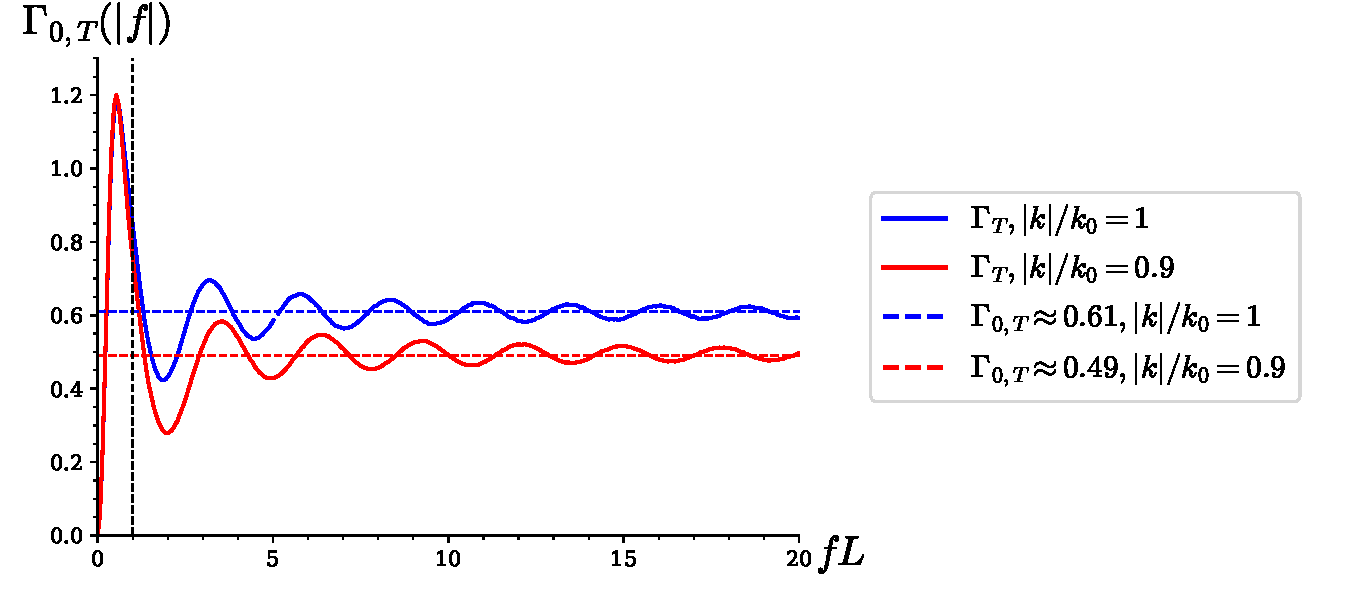
\includegraphics[width=0.8\textwidth]{fig0.pdf}
%    \caption{The frequency-dependent ORF plotted as a function of $fL$. We see that for $fL$ near 1, the ORF is certainly not negligibly different from the frequency-independent value.}
%    \label{fig:freq_dep}
%\end{figure}
We use Monte-Carlo integration to numerically compute the frequency dependence of the effective ORF. The magnitude of $\Gamma_T(|f_{\text{min}}|)$ is significantly greater than $\Gamma_T$ with the factors of $\mathcal{E}(f, \hat{\bf \Omega})$ suppressed. If the ORF is in the regime where the Taylor expansions in the short wavelength ($fL \gg 1$) or long wavelength ($fL \ll 1$) cannot be carried out, then we must not ignore $\mathcal{E}(f, \hat{\bf \Omega})$.
\begin{figure}[ht]
    \centering
    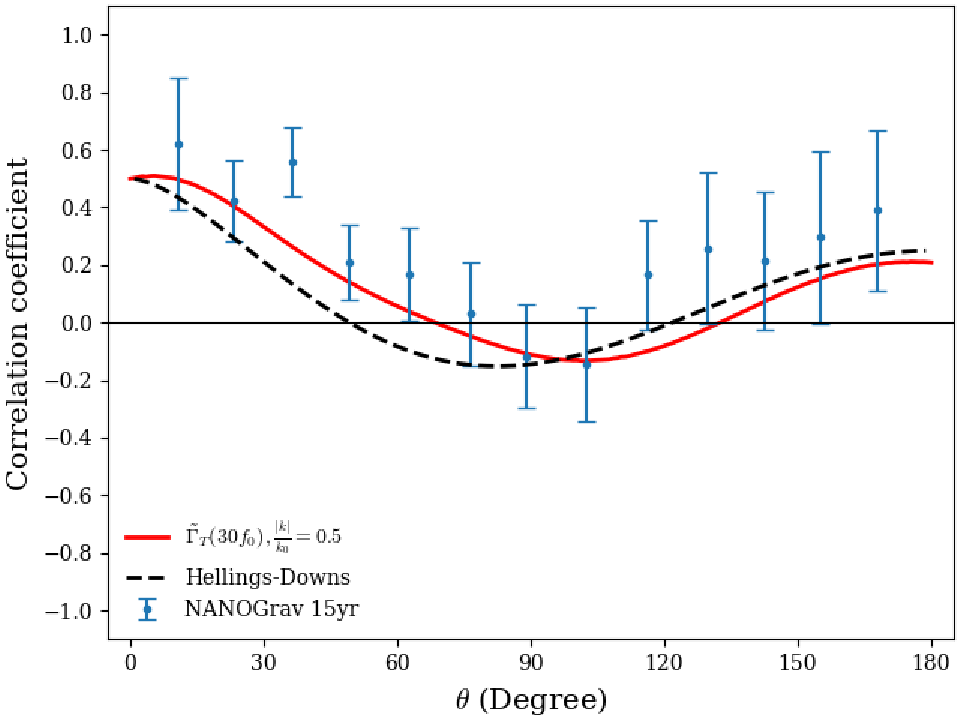
\includegraphics[scale=0.48]{fig1.pdf}
    \caption{The ORFs plotted as a function of angular separation $\xi$. The solid lines use the full expression of the ORFs, including the factors of $\mathcal{E}$. The dotted lines are frequency independent and ignore the factors of $\mathcal{E}$. The solid lines are plotted with $fL = 1$}
    \label{fig:orfs}
\end{figure}
In Fig.\ \ref{fig:orfs}, we see how differently the ORFs behave when we take into account the frequency dependence and when we ignore it. We observe that for a fixed $fL$, the ratio $|{\bf k}|/k_0$ corresponds to an increasing disparity between the frequency-dependent and -independent ORFs. For sufficiently small values of the ratio $|{\bf k}|/k_0$, e.g.\ $|{\bf k}|/k_0 \lesssim 0.1$, the frequency-dependent ORF acquires additional local extrema, namely a minimum and a maximum. This is a peculiarity that only arises when factors of $\mathcal{E}$ are taken into account. We also expect such a drastic behavior to emerge when the mass of the graviton is sufficiently high.
%, which corresponds to the ratio according to 
%\begin{equation}\label{eqn:ratio_m}
%    \frac{|{\bf k}|}{k_0} = \sqrt{1 - \frac{m^2}{k_0^2}}
%\end{equation}

%\subsection{Graviton Mass}\label{subsec:mass}
The graviton mass is intimately connected to the behavior of the effective ORF. It appears as a ratio between the mass and the effective angular frequency.
%, through Eq.\ \ref{eqn:ratio_m}. 
If observations of PTAs follow the trajectory for the best-case scenario, then we can only hope to observe a graviton mass given by that lower frequency bound. This corresponds to $m_g \sim 1.31\times 10^{-24} \eV$. To be clear, we are assuming that the lowest theoretical frequency that we can probe, given by the limit of the dispersion relation as $k\rightarrow 0$, will coincide with the lowest practical frequency that PTAs can measure, hence the ``best-case'' scenario. Going forth, this is the mass that we will take $m_g$ to be in our analysis.

The graviton mass affects all the ORFs for each polarization type, including the tensor modes. The graviton mass shows up in the exponential terms as the coefficient in front of the dot product $\sqrt{1 - (m_g/k_0)^2}\hat{\bf \Omega}\cdot \hat{\bf p}_j$ and in the massive spin-1 helicity-0 polarization vector $\epsilon_\mu^0(m_g) = \sqrt{1 / (1 - (m_g/k_0)^2)}\times (\sqrt{1 - (m_g/k_0)^2},$ $\sin\theta\cos\varphi, \sin\theta\sin\varphi, \cos\theta)$. The former appears in all of the polarization types, but the latter only appears in the vector and scalar modes in the receiving functions, further complicating their mass dependences. The analytical expressions we are integrating can be found in Ref.\ \cite{Liang:2021bct}, except that the expressions we use contain $\mathcal{E}$. Interestingly, because the graviton mass only appears as a ratio $m_g / k_0$, the behavior of the ORF is only sensitive to the mass relative to the frequency. In other words, there is no significance of an ORF purely due to a graviton mass of $m_g$. The question would be, with regard to what frequency?

%\section{Results}\label{sec:results}
\textit{Results}---We now present the main results of this work. Although our calculations are for observations that extend well into the future, it is instructive to compare to current data and confirm whether they are within the present standard deviations, or perhaps explain the current data better than the Hellings-Downs. We compute the full frequency-dependent ORF using the same technique as earlier, i.e.\ Monte-Carlo integration. We keep $m_g$ fixed, and we modify the ratio $|{\bf k}|/k_0$ by changing the frequency $f$ we put into the ORF. We take two characteristic frequencies, one in the first half of the frequency interval (let us call this $f_0$), and one in the second half ($f_1$). This yields ratios of 0.1 and 0.5, respectively. We then compare the resulting effective ORFs with PTA data that it most closely resembles the ORF. For the ORF generated from $|{\bf k}|/k_0 = 0.1$, we compare it against the NANOGrav 15-year dataset \cite{Agazie:2023, Xu:2023wog}, and for the ORF generated from $|{\bf k}|/k_0 = 0.5$, we compare it against the CPTA Data Release I (DR1) \cite{Xu:2023wog}.

We use the NANOGrav 15-yr to obtain the angular correlations of 2,211 pairs of pulsars from a 67-pulsar array \cite{Agazie:2023}. 
\begin{figure}[ht]
    \centering
    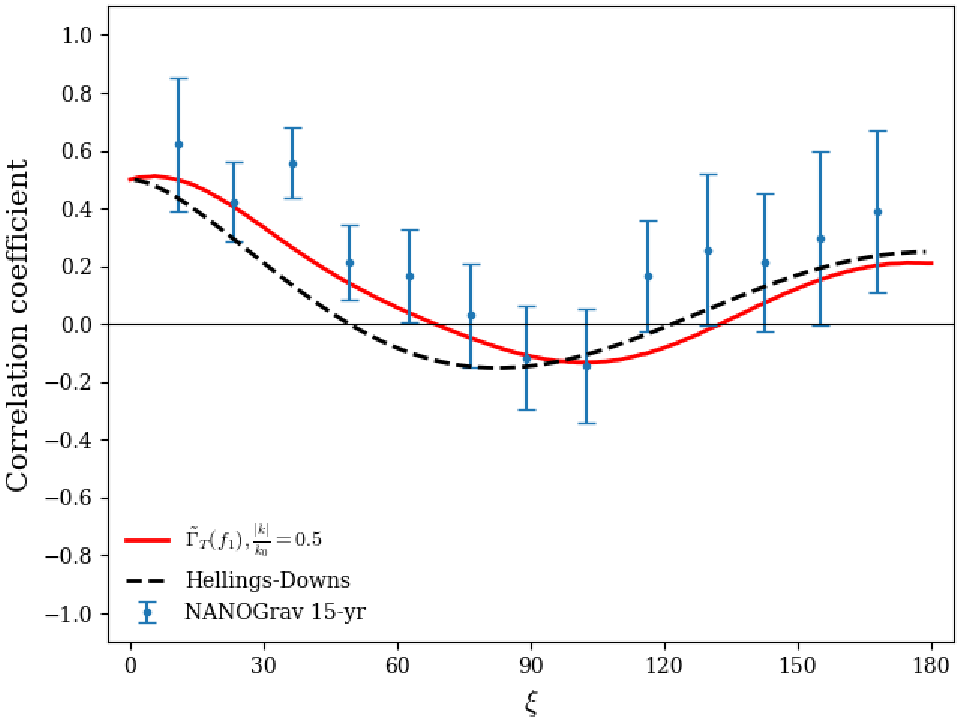
\includegraphics[width=0.45\textwidth]{fig2.pdf}
    \caption{The frequency-dependent effective overlap reduction function plotted in red as a function of the angular separation $\xi$ between a pair of pulsars, in red. This is plotted at the upper frequency, $f_1$, and we set $|{\bf k}|/k_0 = 0.5$. The angular-separation–binned inter-pulsar correlations for the NANOGrav 15-year dataset are plotted with error bars.}
    \label{fig:ng}
\end{figure}
We do not use the frequentist optimal statistic that Ref.\ \cite{Agazie:2023} employs, which is based on methods described in Ref.\ \cite{Allen:2022ksj}, since it is crucial that the estimator is not biased towards the Hellings-Downs. We want the statistics to not assume anything about the additional polarizations, so that our comparison is sensible. For Fig.\ \ref{fig:ng}, we used 13 bins constructed such that the mean of each bin matches the mean $\xi$'s of the CPTA data as closely as possible, since we are not able to alter the number or range of the bins in the CPTA data due to its public inaccessibility. Unfortunately, due to this complication, we compute the statistics for each binned average, rather than the correlation coefficient for each pair, since we want the statistics for the two data sets to be on equal footing. 

We find that for the NANOGrav 15-yr data, the Hellings-Downs gives a fit of $\chi^2$/d.o.f.\ $\sim 1.71$ whereas $\tilde{\Gamma}_T(f_1)$ with $|{\bf k}|/k_0 = 0.5$ gives a fit of $\chi^2$/d.o.f.\ $\sim 1.02$. The effective ORF from MG  is therefore a better fit overall, although it still suffers from not matching the data in the first half of the data.

We use CPTA DR1 to manually reconstruct the binned average values from 1,596 pairs of pulsars of a 57-pulsar array \cite{Xu:2023wog}. 
\begin{figure}[ht]
    \centering
    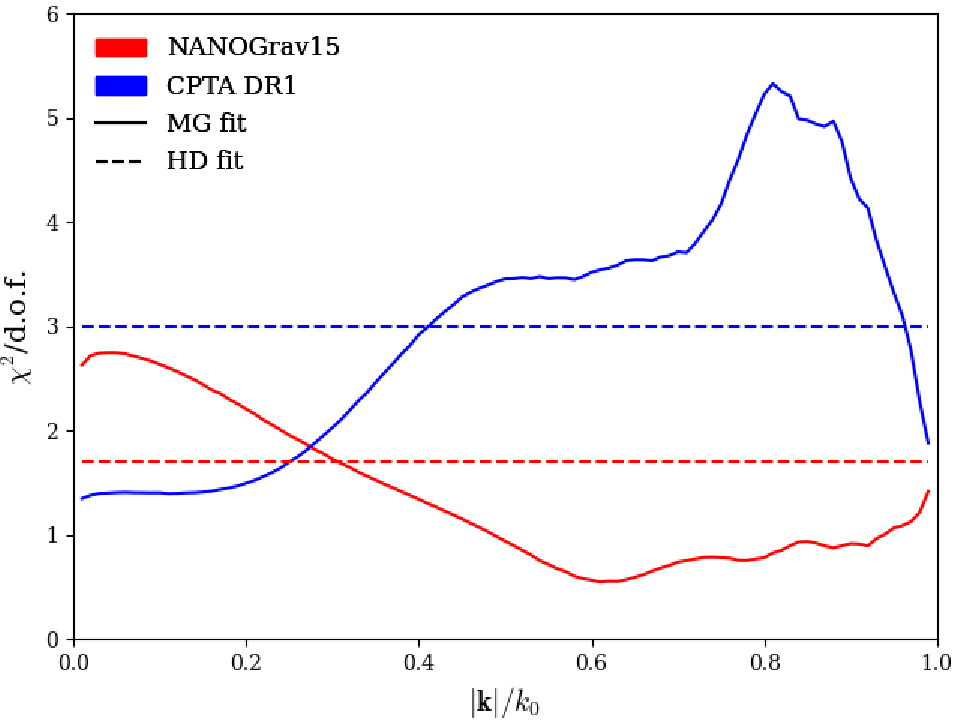
\includegraphics[width=0.45\textwidth]{fig3.pdf}
    \caption{The frequency-dependent effective overlap reduction function plotted as a function of the angular separation $\xi$ between a pair of pulsars, in blue. This is plotted at the lower bound of the frequency, $1/T_{\text{CTPA}}$, and we set $|{\bf k}|/k_0 = 0.1$. The angular–separation–binned inter-pulsar correlations for the CPTA dataset for $1/T_{\text{CTPA}}$ are plotted with error bars.}
    \label{fig:cpta}
\end{figure}
This dataset is chosen because of the frequency dependence that the CPTA collaboration noted \cite{Xu:2023wog}, and due to the peculiar shape of the data. The CPTA collaboration has done an analysis on the correlation coefficients for the frequencies $1/T_{\text{CTPA}}, 1.5/T_{\text{CTPA}},$ and $2/T_{\text{CTPA}}$, where $T_{\text{CTPA}} \sim 3.40$ years. We use the data for $1/T_{\text CTPA}$ since it is closer to $f_0$, which we wish to analyze. 

We find that for CPTA DR1, the Hellings-Downs gives a fit of $\chi^2$/d.o.f.\ $\sim 3.00$ whereas $\tilde{\Gamma}_T(f_0)$ with $|{\bf k}|/k_0 = 0.1$ gives a fit of $\chi^2$/d.o.f.\ $\sim 1.51$. The effective ORF from MG  is a significantly better fit than the Hellings-Downs. In fact, the effective ORF from MG does remarkably well in matching the data. We summarize our statistics in Table \ref{tbl:chi}.
\begin{table}[ht] 
\centering
\renewcommand{\arraystretch}{1.8}
\begin{tabular}{|c|c|c|c|}
\hline
\textbf{Data} & \textbf{Fit} & \textbf{$\chi^2$} & \textbf{$\chi^2$/d.o.f.} \\
\hline
NANOGrav 15-yr & Hellings-Downs & 22.20 & 1.71 \\
\hline
NANOGrav 15-yr & MG  & 11.22 & 1.02 \\
\hline
CPTA DR1 & Hellings-Downs & 38.95 & 3.00 \\
\hline
CPTA DR1 & MG  & 16.58 & 1.51 \\
\hline
\end{tabular}
\caption{The $\chi^2$ and $\chi^2$/d.o.f.\ values for different fit functions for the two datasets used in this analysis. We have 13 degrees of freedom for the Hellings-Downs correlation and 11 for the MG  models, with 2 fit parameters: $m_g$ and $f$. }
\label{tbl:chi}
\end{table}

%\section{Discussion}\label{sec:discussion}
\textit{Discussion and conclusion}---In this paper, we have reviewed the methods for obtaining the modified dispersion relation and effective ORF in the theory of ghost-free massive gravity. We have analyzed the behavior of this effective ORF when the exponential factors are not ignored. We were able to demonstrate using unbiased NANOGrav 15-yr data and CPTA DR1 that the effective ORF in MG fits the data significantly better than the Hellings–Downs with an optimistic graviton mass $m_g \sim$ $1.31\times10^{-24} \eV$.

%Our findings show that MG  is able to explain the observed pulsar-pulsar correlation more convincingly than the Hellings-Downs. 
In this Letter, we have not performed a rigorous fitting of the data; we simply used characteristic frequencies for comparison. A rigorous fitting to the full data in a different context has been done in Ref.\ \cite{Arjona:2024cex}, and the ratio that has been found to best fit the frequentist optimal statistic of the NANOGrav 15-yr data is $|{\bf k}|/k_0 \sim 0.73$. We deem this to be plausible, based on our statistics and the resulting shape of our ORF. A future study may introduce more free parameters than the ones we considered and perform a holistic fitting procedure to place constraints on the mass of the graviton and its relative energy densities. Additionally, it would be of use to perform the fitting on the individual pulsar-pulsar correlation coefficients rather than the binned averages, if such data can be obtained for CPTA or other collaborations. 
%Our analysis explores the novel possibility of incorporating the exponential factors in the ORFs. For most pulsars considered in PTA experiments, the exponential factors can be safely ignored because of the large distances involved with them, but for a substantial portion of the pulsars, $fL$ will be less than 10. It is crucial that we understand how $\mathcal{E}$ affects the ORF in these cases. We have observed new extrema that appear in cases where the observed frequency is sufficiently low or the graviton mass is sufficiently high. For a more thorough analysis, we can calculate the ORF for every single pulsar pair with their true $L_1$ and $L_2$ values, and see how this diverges from the ORF when $\mathcal{E}$ is ignored.

An assumption we made previously is that the stochastic GW background is isotropic. It is what allows us to decompose Eq.\ \ref{eqn:two_point_z} in the way that we did, but it is not necessarily an assumption we can take for granted \cite{Depta:2024ykq, Bravo:2025csu, Cusin:2025xle, Kuwahara:2024jiz, Li:2024lvt}. Anisotropy in the background can be analyzed by decomposing the ORF in the basis of spherical harmonics and analzying the multipole moments associated with these harmonics \cite{Allen:2024bnk, Gair:2014rwa}\footnote{It may not be appropriate to do spherical harmonic decomposition for the analysis of realistic PTAs \cite{Ali-Haimoud:2020ozu}. Instead, the Fischer formalism may be more effective, especially in the context of anisotropic backgrounds.}. This can be applied to the effective ORFs we have derived and may be of interest in further work. 
%It is an approach we have briefly considered for our analysis of the ORFs, but ultimately had to abandon in order to pursue an alternative approach.

Analyzing the frequency dependence of the ORF in general is underexplored. The NANOGrav collaboration and other PTA collaborations do not claim to detect any frequency dependence in the ORF, while the CPTA collaboration has. If the graviton is massive, then there will certainly be frequency dependence in the data, even without considering $\mathcal{E}$. Doing an analysis of the frequency dependence of the NANOGrav data would therefore be quite elucidative. 
%It is beyond the scope of this paper to perform such an analysis.

The detection prospects suggested in this Letter are quite optimistic. It may be unlikely that we see a PTA experiment last that long, but we nevertheless provide a detailed overview of the ORFs that we may observe if such a scenario takes place. Regarding data from current PTA collaborations, the prospects seem hopeful of continuing to detect pulsar-pulsar correlation coefficients such that the ORFs generated in a theory of MG  stay within their standard deviations. With more galactic pulsars being added to PTAs and the planned missions of space-based GW observatories (LISA and Taiji) on the horizon, it seems plausible that the mysteries that have evaded our investigations surrounding the cosmos may finally start to be unravelled. Clearly, a new era of GW observations is well underway. 

We conclude with the notion that these results are not dependent on the astrophysical origins of the stochastic GW background. If gravitons are massive, then they will behave according to the principles laid out in this Letter, and we should expect to see the effects of this appear in various observables, regardless of whether the source is composed of continuous signals from supermassive black hole binaries or primordial GWs generated during inflation.

\vspace{5mm}
\textit{Acknowledgements}---We thank Qiuyue Liang, Neil Cornish, and Murman Gurgenidze for useful discussions related to the paper. We also thank the organizers of the 2025 Phenomenology Symposium (PHENO), during which much of this paper has been developed. C.C.\ and T.K.\ acknowledge support from the NASA Astrophysics Theory Program (ATP) Award 80NSSC22K0825 and the National Science Foundation (NSF) Astronomy and Astrophysics Research Grants (AAG) Award AST2408411.

\vspace{5mm}
\textit{Data availability}---The NANOGrav 15-year data used in this paper are publicly available at NANOGrav. Source code to reproduce all of our results (figures and Table \ref{tbl:chi}) is available in our GitHub repository \href{https://github.com/ChrisChoi314/graviton_mass_ORF}{graviton\_mass\_ORF}.

\bibliographystyle{apsrev4-2_edited}
\bibliography{refs}


\clearpage
\end{document}
